Одной из задач в данном семестре было написание плагина сбора сохраненных логинов и паролей для браузера Mozilla Firefox.

Сохраненные логины и пароли хранятся в папке с профилем Mozilla Firefox. Путь к папке: C:\textbackslash Users\textbackslash User\textbackslash AppData\textbackslash Roaming\textbackslash Mozilla\textbackslash Firefox\textbackslash Profiles\textbackslash prof\_n. Где prof\_n генерируется самим браузером.

Для браузеров, версия которых 31 и меньше, логины и пароли хранятся в файле базы данных signons.sqlite. База данных имеет формат sqlite3. В базе данных есть таблица moz\_logins. Интересующие столбцы: encryptedUsername, encryptedPassword, formSubmitURL, которые содержат зашифрованный логин, зашифрованный пароль и URL сайта соответственно.

Для остальных, логины и пароли хранятся в файле logins.json.

Json – текстовый формат файла, в котором информация представлена в виде структур. На рисунке~\ref{teresh_1:teresh_1} показано, как выглядит файл logins.json.

\begin{figure}[h!]
\center{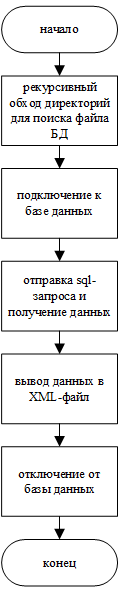
\includegraphics[width=0.9\linewidth]{teresh_1}}
\caption{Файл logins.json}
\label{teresh_1:teresh_1}
\end{figure}

Здесь интересны те же поля, как и в случае с базой данных.

Как видно из рисунка~\ref{teresh_1:teresh_1}, логины и пароли зашифрованы. Для их расшифровки необходимы файлы cert8.db, key3.db и secmod.db. В них содержатся ключи для расшифровки значений. Эти файлы также находятся в папке с профилем.

Так же для работы модуля необходима библиотека nss3. Именно с помощью нее браузер зашифровывает логины и пароли.

Nss3 – open source библиотека, разработанная для создания кроссплатформенных защищенных клиентских и серверных приложений.

\subsubsection{Алгоритм работы плагина}

Сначала модуль подключает стороннюю библиотеку nss3. Затем выполняется поиск файла compatibility.ini (также находится в папке профиля), содержащего версию браузера.

Для браузеров, версия которых 31 и меньше, ищется файл базы данных signons.sqlite. Модуль подключается к нему и выполняет sql-запрос: <<SELECT encryptedUsername, encryptedPassword, formSubmitURL FROM moz\_logins>>.

Для других версий, ищется файл logins.json, вытаскиваются нужные нам значения.

Затем данные расшифровываются с помощью сторонней библиотеки nss3 и сохраняются в xml-файл.

Блок-схема программы представлена на рисунке~\ref{teresh_2:teresh_2}.

\begin{figure}[h!]
\center{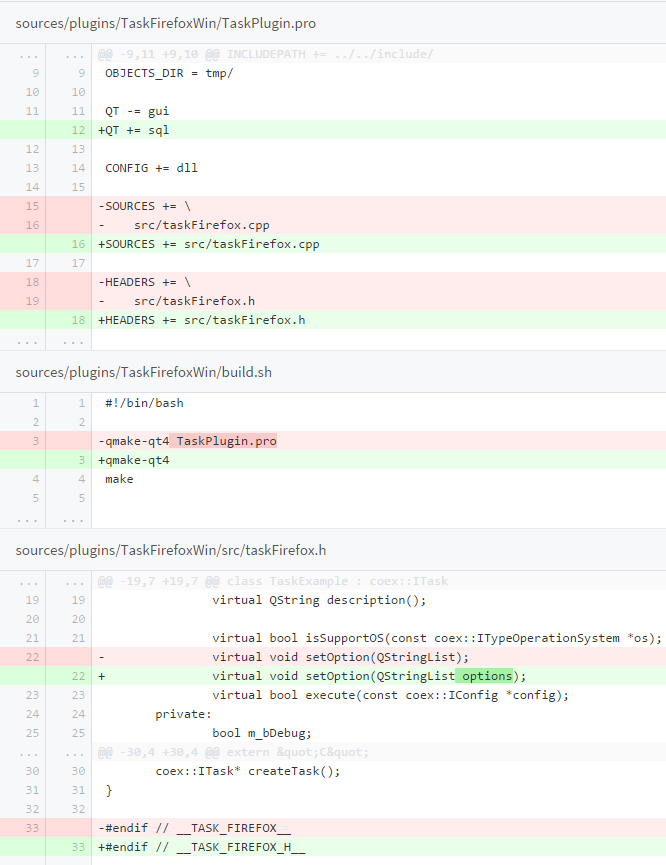
\includegraphics[width=0.6\linewidth]{teresh_2}}
\caption{Алгоритм работы плагина}
\label{teresh_2:teresh_2}
\end{figure}

\subsubsection{Тестирование}

Как видно из рисунков~\ref{teresh_3:teresh_3} и~\ref{teresh_4:teresh_4} плагин выполняет поставленные перед ним задачи.

\begin{figure}[h!]
\center{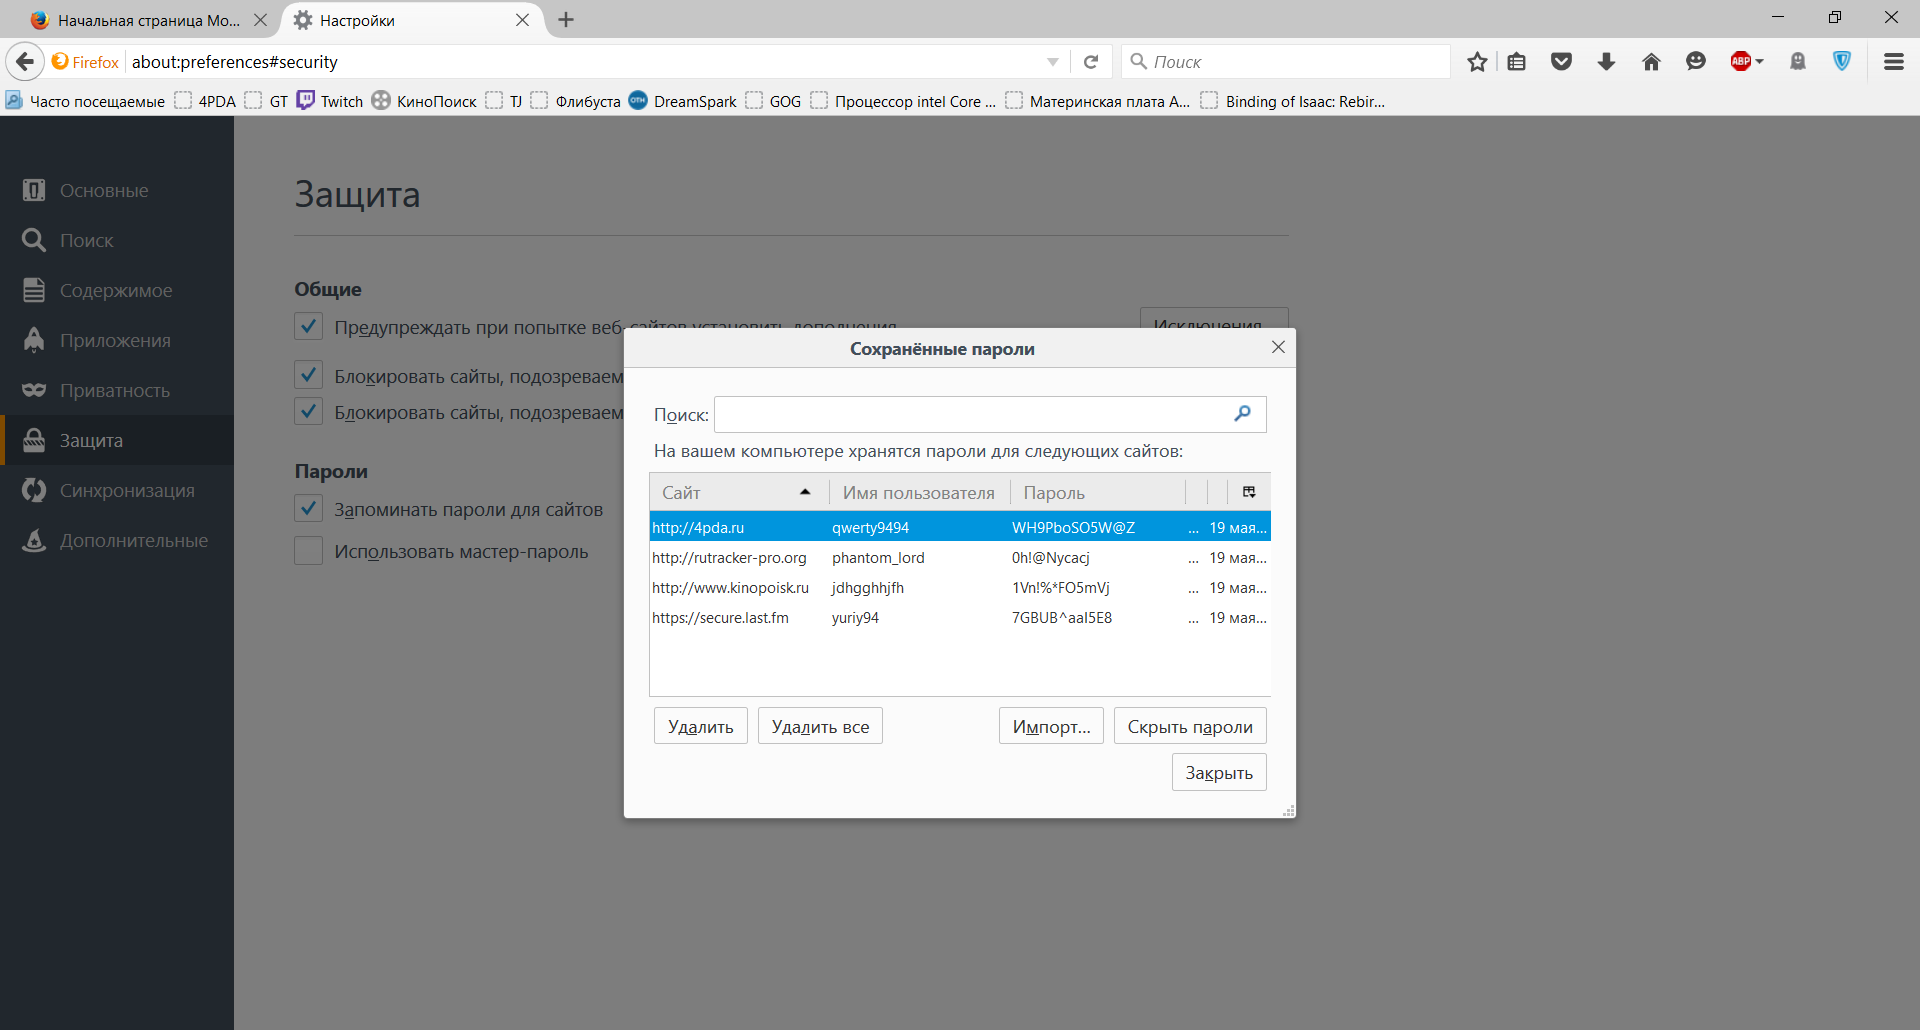
\includegraphics[width=1\linewidth]{teresh_3}}
\caption{Тестовые данные}
\label{teresh_3:teresh_3}
\end{figure}

\clearpage
\begin{figure}[h!]
\center{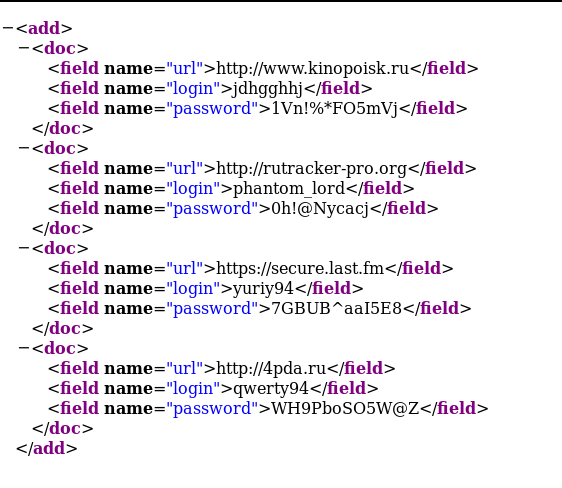
\includegraphics[width=0.7\linewidth]{teresh_4}}
\caption{Результат тестирования}
\label{teresh_4:teresh_4}
\end{figure}

\clearpage
